\documentclass{beamer}
\usecolortheme{whale}

\usepackage[utf8]{inputenc}

\usepackage{graphicx}
\usebackgroundtemplate%
{%
    
\includegraphics[width=\paperwidth]{Images/fondodocker}%
}

\title{Primeros pasos con Docker}
\author{Víctor Orozco}
\institute{Nabenik}
\date{\today}

\begin{document}

\frame{\titlepage}

\section{Intro}

\begin{frame}{VMs}
\begin{figure}
\centering

\includegraphics[width=0.7\linewidth]{Images/virtualbox}
\label{fig:vm}
\end{figure}
\end{frame}

\begin{frame}{Hipervisores}
\begin{figure}
\centering
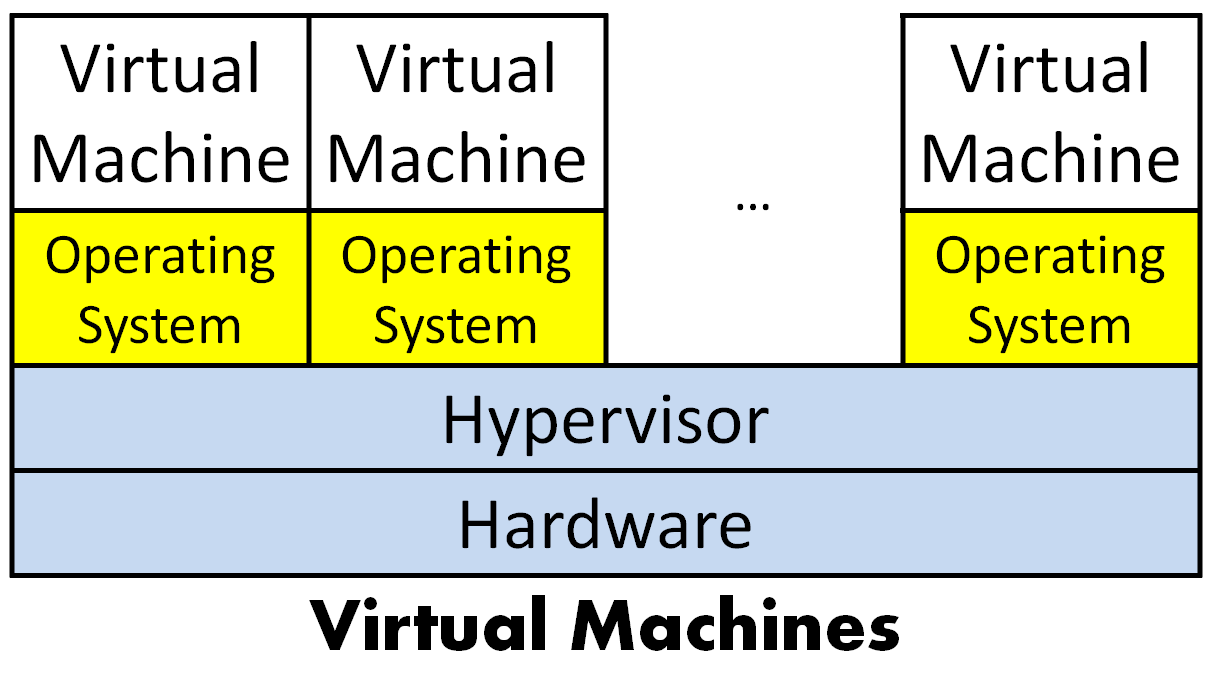
\includegraphics[width=0.7\linewidth]{Images/hypervisors}
\label{fig:hypervisors}
\end{figure}
\end{frame}

\begin{frame}{VM/Hipervisores}
VM
\begin{itemize}
\item VirtualBox
\item VMWare Player
\item MS Virtual Pc
\end{itemize}
Hipervisores
\begin{itemize}
\item Xen
\item KVM
\end{itemize}
\end{frame}

\begin{frame}{Despliegue tradicional}
\begin{figure}
\centering
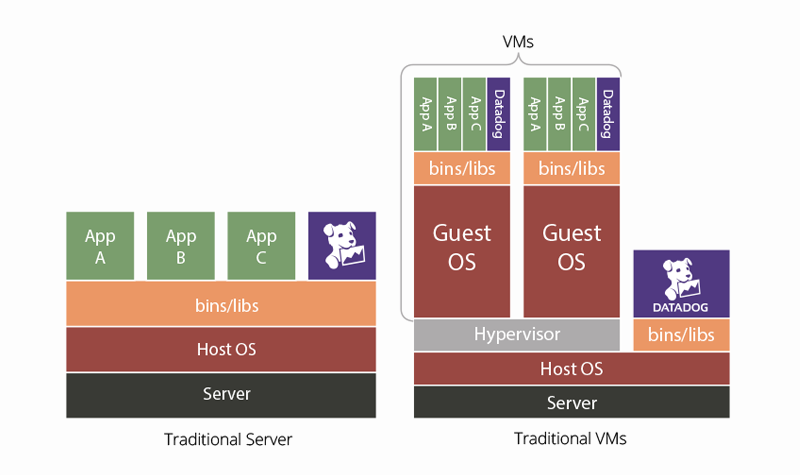
\includegraphics[width=0.8\linewidth]{Images/traditional}
\label{fig:traditional}
\end{figure}
\end{frame}

\begin{frame}{Despliegue contenedores}
\begin{figure}
\centering
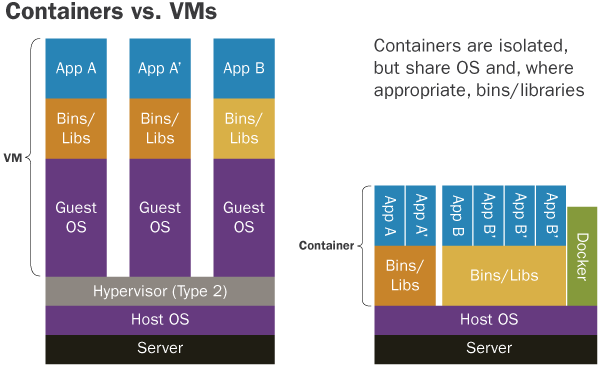
\includegraphics[width=0.8\linewidth]{Images/containervsvm.png}
\label{fig:containervsvm}
\end{figure}
\end{frame}

\begin{frame}{Contenedor}
Contenedor = bibliotecas + app + shell
\begin{figure}
\centering
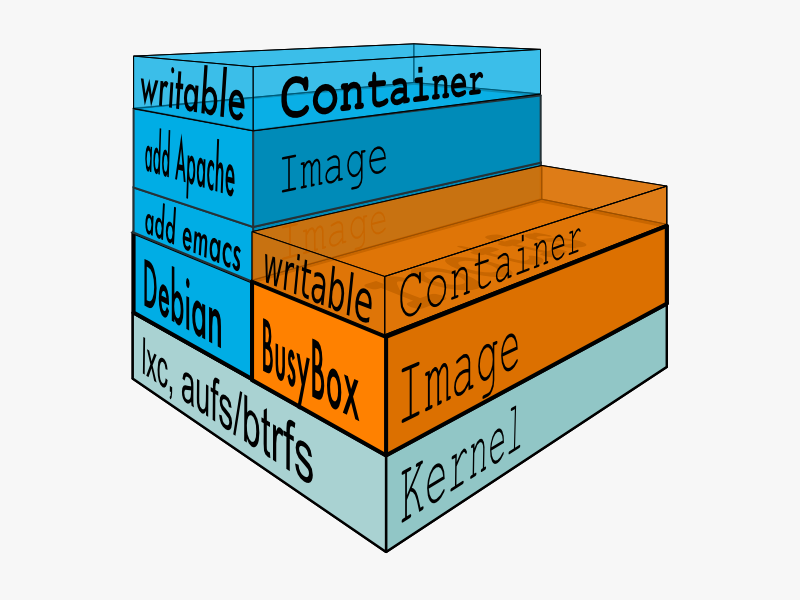
\includegraphics[width=0.8\linewidth]{Images/container.png}
\label{fig:container}
\end{figure}
\end{frame}

\begin{frame}{Docker}
\begin{itemize}
\item Cgroups + Namespace: Isolamiento de recursos de un grupo y visibilidad entre procesos
\item libcontainer (LXC/Libvirt/systemd-nspawn)
\item SELinux, AppArmor, Netfilter
\pause\item Ventajas: Boot time, menos overhead
\pause\item Desventajas: Ecosistema joven (aka pocas GUI), Linux \pause (meh!)
\end{itemize}
\end{frame}

\begin{frame}{Hands-On}
\begin{itemize}
\item docker version
\item docker images
\item docker search -image-
\item docker pull -image-
\end{itemize}
\end{frame}

\begin{frame}{Hands-On}
\begin{figure}
\centering
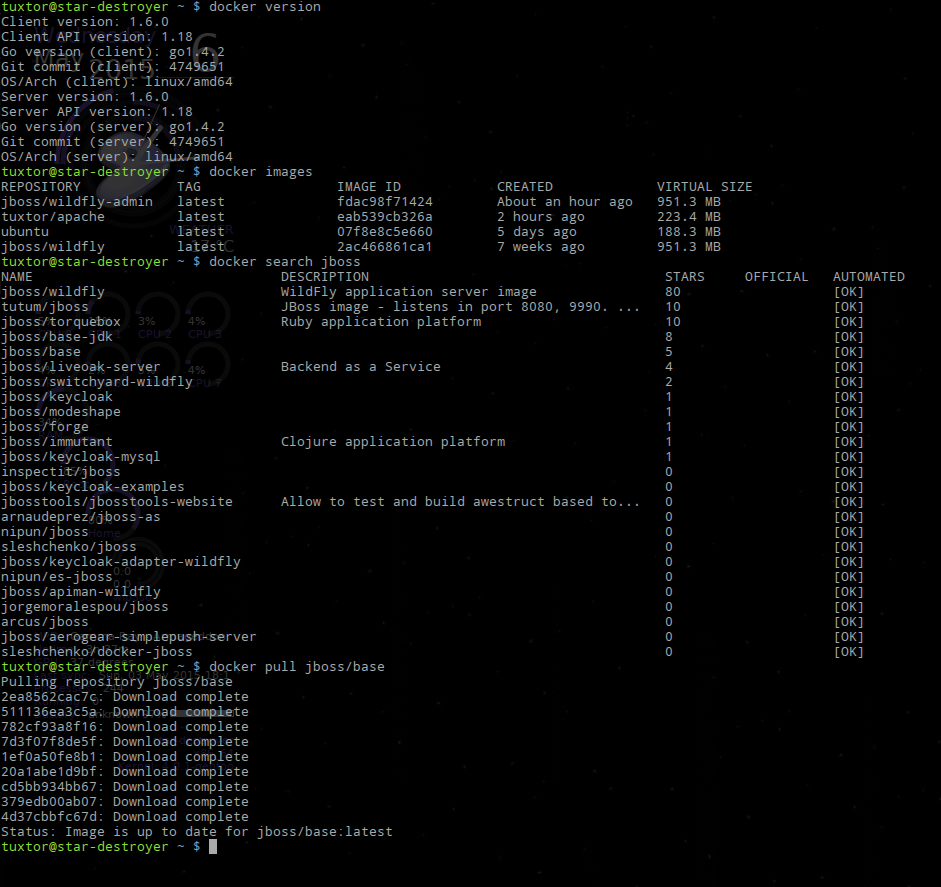
\includegraphics[width=0.8\linewidth]{Images/handson.png}
\label{fig:handson}
\end{figure}
\end{frame}


\begin{frame}{Demo 1}
\begin{itemize}
\item Imagen base (ubuntu)
\item Ejecución
\item Agregar paquete
\item Commit
\item Ejecución
\end{itemize}
\end{frame}

\begin{frame}{Demo 1}
\begin{itemize}
\item docker pull ubuntu
\item docker run ubuntu echo "Hola ubuntu"
\item docker run -it ubuntu /bin/bash
\item apt-get update\&\&apt-get install apache
\item docker ps
\item docker commit -id- tuxtor/apache
\item docker run -it tuxtor/apache /bin/bash
\end{itemize}
\end{frame}

\begin{frame}{Demo 2}
\begin{itemize}
\item App Java Web (usac-web)
\item Imagen base (jboss/wildfly)
\item Dockerfile
\item Tag
\item Ejecución
\end{itemize}
\end{frame}

\begin{frame}{Complementos}
\begin{itemize}
\item Vagrant boxes
\item Kubernets
\item CoreOS
\item etcd
\end{itemize}
\end{frame}

\section{Fin}

\begin{frame}{Gracias}
\begin{itemize}
\item tuxtor@shekalug.org
\item http://tuxtor.shekalug.org
\item http://github.com/tuxtor/slides
\end{itemize}
\begin{center}

\includegraphics[width=0.1\linewidth]{Images/cclogo}
\\
This work is licensed under a Creative Commons Attribution-ShareAlike 3.0 Guatemala License.
\end{center}
\end{frame}
\end{document}
